% !TeX spellcheck = pl_PL

\rozdzial

%%%%%%%%%%%%%%%%%%%%%%%%%%%%%%%%%%%%%%%%%%%%%%%%%%%%%%%%%%%%%%%%%%%%%%%
\section{Biuro}
\label{biuro}

\begin{figure}[htb]
	\centering
	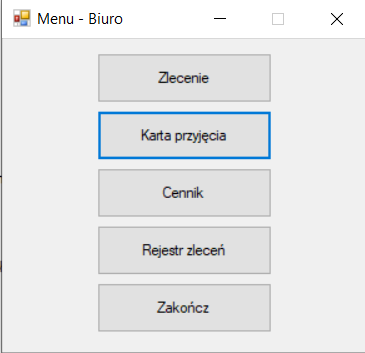
\includegraphics{obrazki/Biuro/menu_biuro.png}
	\caption{Menu części biurowej.}
	\label{menuBiuro}
\end{figure}

\subsection{Zlecenie}
\label{zlecenie}

\subsection{Karta przyjęcia}
\label{karta_przyjecia}

\begin{figure}[htb]
	\centering
	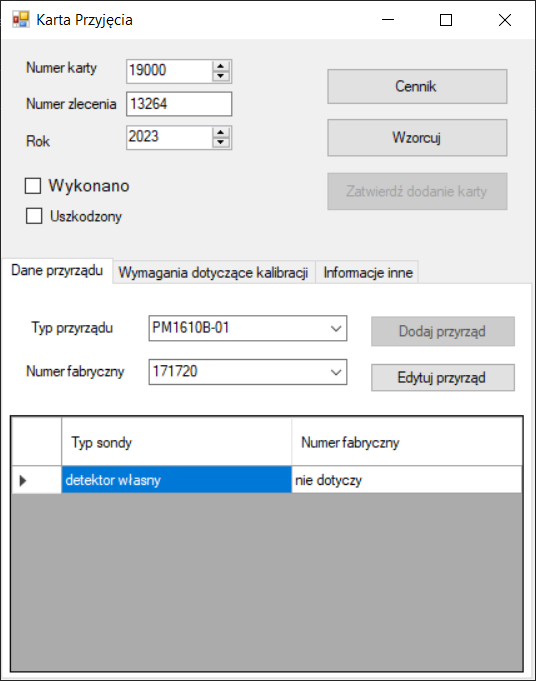
\includegraphics{obrazki/Biuro/karta/karta_dane_przyrzadu.png}
	\caption{Karta przyjęcia - zakładka z danymi przyrządu.}
	\label{kartaDanePrzyrzadu}
\end{figure}

\begin{figure}[htb]
	\centering
	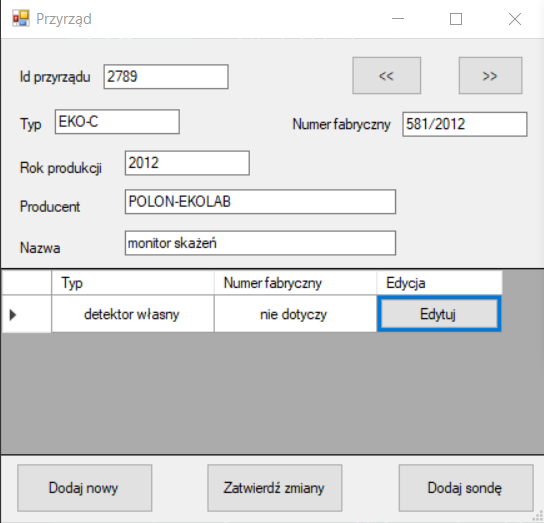
\includegraphics{obrazki/Biuro/karta/edytuj_przyrzad.png}
	\caption{Okno edycji danych przyrządu.}
	\label{edytujPrzyrzad}
\end{figure}

\begin{figure}[htb]
	\centering
	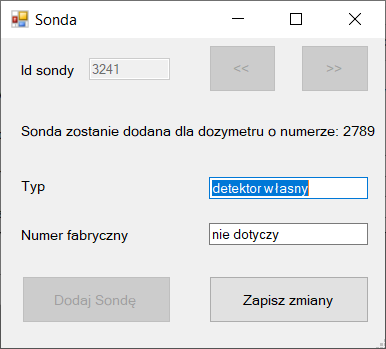
\includegraphics{obrazki/Biuro/karta/edytuj_sonde.png}
	\caption{Okno edycji sondy.}
	\label{edytujSonde}
\end{figure}

\begin{figure}[htb]
	\centering
	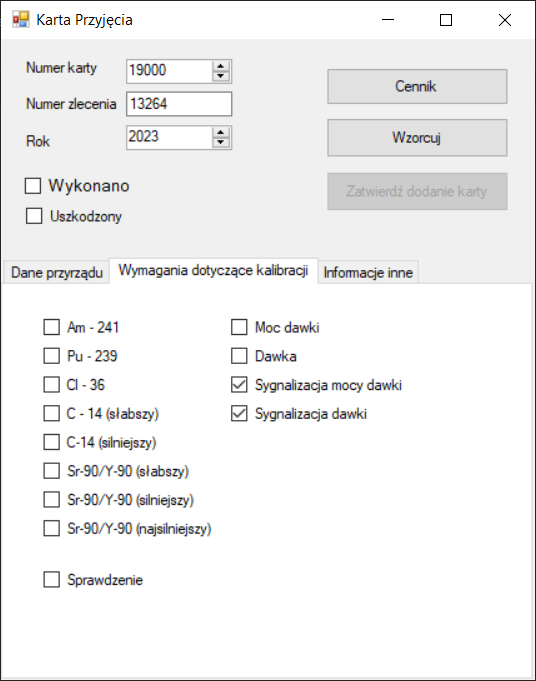
\includegraphics{obrazki/Biuro/karta/karta_dane_wymagania.png}
	\caption{Karta przyjęcia - zakładka z informacjami o danych dotyczących kalibracji.}
	\label{kartaDaneKalibracji}
\end{figure}

\begin{figure}[htb]
	\centering
	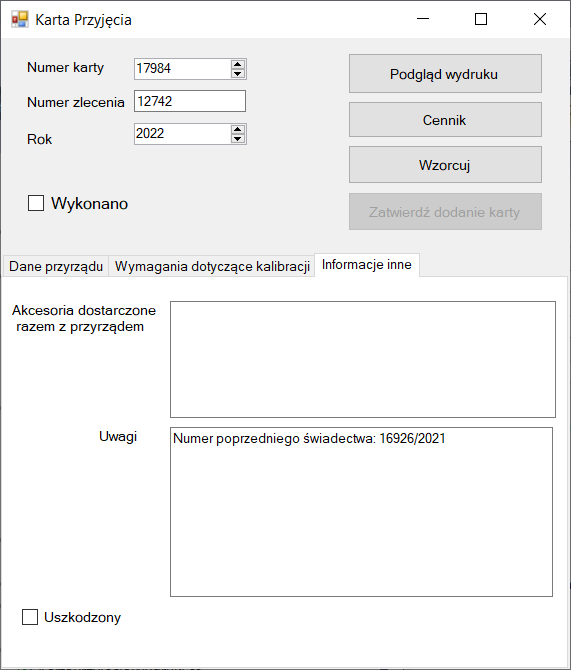
\includegraphics{obrazki/Biuro/karta/karta_dane_inne.png}
	\caption{Karta przyjęcia - zakładka z pozostałymi danymi.}
	\label{kartaDaneInne}
\end{figure}


\subsection{Cennik}
\label{cennik}

\begin{figure}[htb]
	\centering
	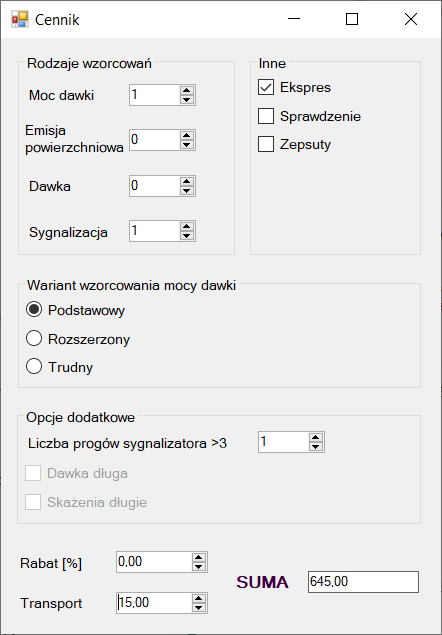
\includegraphics{obrazki/Biuro/cennik.png}
	\caption{Okno cennika}
	\label{cennikRys}
\end{figure}

\subsection{Rejestr zleceń}
\label{rejestr}

\begin{figure}[htb]
	\centering
	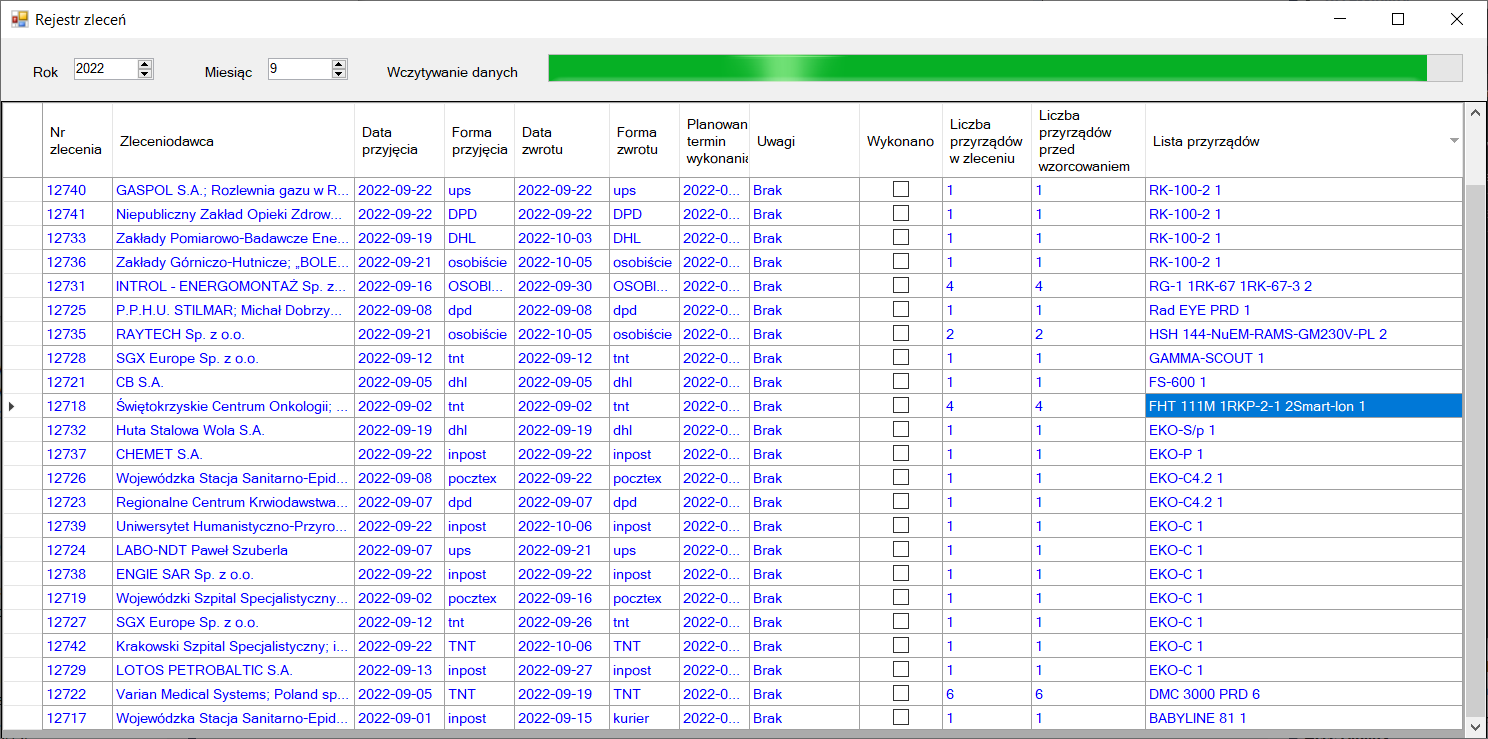
\includegraphics{obrazki/Biuro/rejestr_zlecen.png}
	\caption{Rejestr zleceń}
	\label{rejestrZlecen}
\end{figure}